\subsubsection{Set 1 - Greenyard Maaseik}
\label{sec:PL1_Greenyard1}
%TODO: tekst aanpassen
De opslagen en recepties van de eerste set van Greenyard Maaseik worden weergeven in figuur  \ref{fig:PL1ServeMaaseik1}. De beoordeling van de opslag is op een andere wijze gedaan dan bij de manuele invoer. Bij de manuele invoer wordt er gebruik gemaakt van tekens, terwijl bij de AI-invoer gebruik wordt gemaakt van cijfers. Bij de opslag komt het teken \# overeen met 0, + en / met 1, ! met 2, - en = met 3.

Hier valt op dat de goede opslagen door beide in deze set niet zijn genoteerd. De AI-invoer heeft de opslagen meer verdeeld onder score 1 en 2. Terwijl de manuele invoer enkel score 1 of 3 heeft gegeven. De scouter is dus kritischer in zijn beoordeling van de opslag.

De manuele invoer heeft de recepties beoordeeld met de tekens \# overeen met 3, + en / met 2, ! met 1, - en = met 0.

Bij de receptie zijn er grote verschillen aanwezig tussen de manuele invoer en de AI-invoer. Er is één receptie van Landon Douglas Currie die door de AI-invoer niet kon beoordeeld worden, maar ook hier kan er geconstateerd worden dat de manuele invoer veel kritischer is in zijn beoordeling. 

\begin{figure}[ht]
\centering
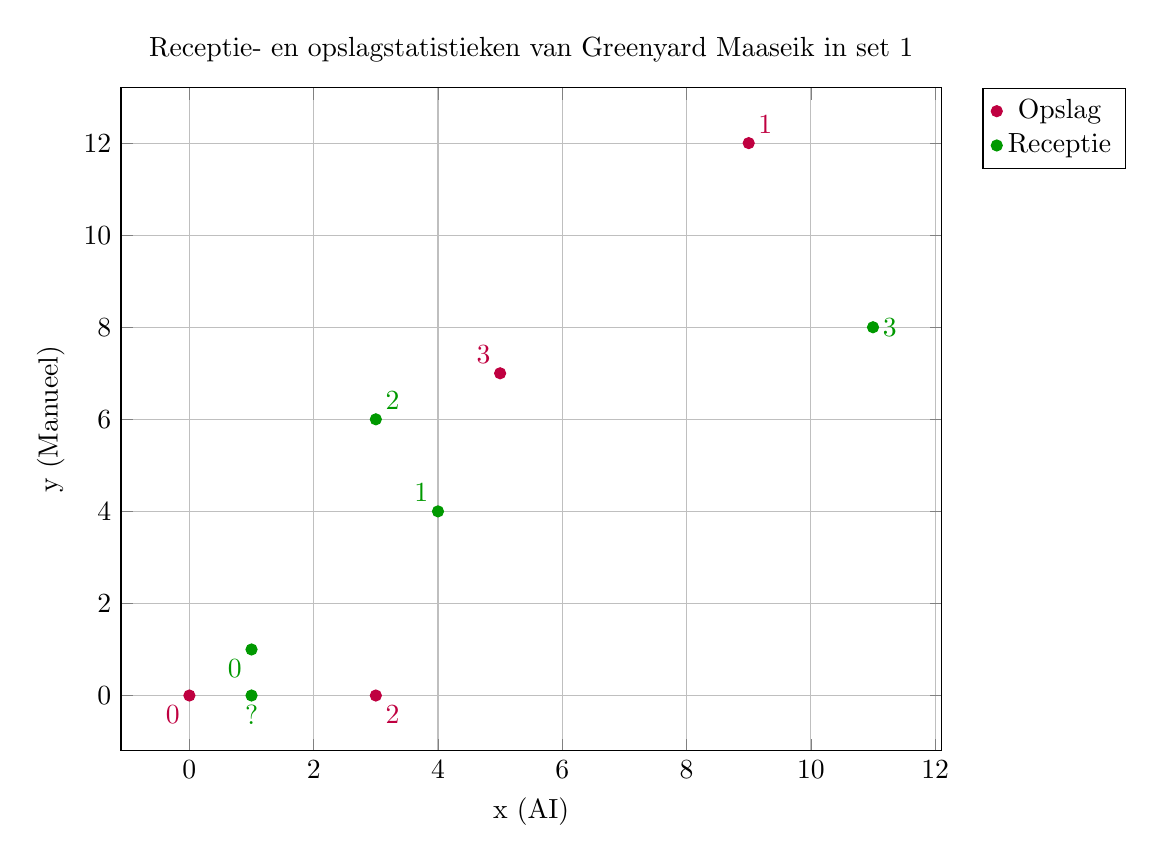
\begin{tikzpicture}
  \begin{axis}[
    title={Receptie- en opslagstatistieken van Greenyard Maaseik in set 1},
    xlabel={x (AI)},
    ylabel={y (Manueel)},
    grid=major,
    legend style={at={(1.05,1)}, anchor=north west},
    width=12cm,
    height=10cm,
    enlargelimits=0.1,
  ]

  % Opslag
  \addplot[
    only marks,
    mark=*,
    color=purple,
  ] table {
    x y
    0 0
    9 12
    3 0
    5 7
  };
  \addlegendentry{Opslag}

  % Labels opslag
  \node at (axis cs:0,0) [anchor=north east, purple] {0};
  \node at (axis cs:9,12) [anchor=south west, purple] {1};
  \node at (axis cs:3,0) [anchor=north west, purple] {2};
  \node at (axis cs:5,7) [anchor=south east, purple] {3};

  % Receptie
  \addplot[
    only marks,
    mark=*,
    color=green!60!black,
  ] table {
    x y
    11 8
    3 6
    4 4
    1 1
    1 0
  };
  \addlegendentry{Receptie}

  % Labels receptie
  \node at (axis cs:11,8) [anchor=west, green!60!black] {3};
  \node at (axis cs:3,6) [anchor=south west, green!60!black] {2};
  \node at (axis cs:4,4) [anchor=south east, green!60!black] {1};
  \node at (axis cs:1,1) [anchor=north east, green!60!black] {0};
  \node at (axis cs:1,0) [anchor=north, green!60!black] {?};

  \end{axis}
\end{tikzpicture}
\caption{AI invoer versus manuele invoer, ingedeeld in opslag en receptie, voor Greenyard Maaseik in set 1.}
\label{fig:PL1ServeMaaseik1}
\end{figure}

De spelverdeling wordt weergegeven in tabellen \ref{tab:PL1SetMaaseikMan1} en \ref{tab:PL1SetDigMaaseikAI1}. Over het algemeen zijn de hoeveelheden van de spelverdeling correct, bij één speler is er een verschil van 1 bij de AI-invoer. De kwaliteit van de set wordt bij de AI niet beoordeeld, waardoor geen verdere vergelijking mogelijk is.

Bij de verdeding, tabel \ref{tab:PL1DigMaaseikMan1} en \ref{tab:PL1SetDigMaaseikAI1}, zijn er duidelijke verschillen te zien. Dig Error (DE) komt overeen met een = bij de manuele invoer. Bij 2 spelers komt dit perfect overeen met de manuele invoer, bij de andere is er echter wel een verschil.  Zij hebben meer of minder verdedigingen gekregen door de AI.

\begin{table}[ht!]
    \centering
    \scriptsize
    \begin{tabular}{|l|c|c|c|c|c|c|c|c|c|} \hline
        \textbf{Speler}& *E\% & Tot & = & / & - & ! & + & \# \\ \hline
        Renet Vancker  & 100\% & 7 &  &  &  &  & 6 & 1  \\
        Jolan Cox  & 100\% & 1 &  &  &  &  & 1 &  \\ 
        Dawid Pawlun  & 100\% & 14 &  &  &  &  & 13 & 1  \\ 
        Pierre Perin & 100\% & 2 &  &  &  &  & 2 & \\ \hline
    \end{tabular}
    \caption[Manueel ingevoerde spelverdelingsstatistieken voor Greenyard Maaseik in set 1]{\label{tab:PL1SetMaaseikMan1}Manueel ingevoerde spelverdeling statistieken voor Greenyard Maaseik in set 1.}
\end{table}

\begin{table}[ht!]
    \centering
    \scriptsize
    \begin{tabular}{|l|c|c|c|c|c|c|c|c|c|} \hline
        \textbf{Speler}  & *E\% & Tot & = & / & - & ! & + & \# \\ \hline
        Thomas Neyens & 0 & 1 & & & & 1 & & \\
        Jolan Cox & 0\% & 2 & 1 &  & 1 &  &  &  \\ 
        Landon Douglas Currie & 100\% & 1 &  &  &  &  & 1 &  \\ 
        Dawid Pawlun & 100\% & 1 &  &  &  &  & 1 &  \\ 
        Miquel Angel Fornés & 100\% & 1 &  &  &  &  & 1 &  \\ 
        Hampus Ekstrand & 0\% & 4 & 3 &  & 1 &  &  &  \\ 
        Pierre Perin & 50\% & 2 & 1 &  &  &  & 1 &  \\ \hline
    \end{tabular}
    \caption[Manueel ingevoerde verdedigingsstatistieken voor Greenyard Maaseik in set 1]{\label{tab:PL1DigMaaseikMan1}Manueel ingevoerde verdedigingsstatistieken voor Greenyard Maaseik in set 1.}
\end{table}

\begin{table}[ht!]
  \centering
  \scriptsize
  \begin{tabular}{|l|c|c|c|c|c|c|c|}  \hline
    \textbf{Speler} & Ast & TA & SE & PCT & DS & DE \\ \hline
    Renet Vancker & 4 & 7 &  & 57\% &  &  \\
    Thomas Neyens &  &  &  &  & 1 &  \\
    Jolan Cox &  & 1 &  & 0\% & 1 & 1 \\
    Landon Douglas Currie &  &   &  &  & 1 &  \\
    Dawid Pawlun & 6 & 13 &  & 46\% & 1 &  \\
    Miquel Angel Fornés &  &  &  &  & 1 & 1 \\
    Hampus Ekstrand &  &  &  &  & 3 & 1 \\
    Pierre Perin &  & 2 &  & 0\% & 1 &  \\ \hline
  \end{tabular}
  \caption[Spelverdelings- en verdedigingsstatistieken gemaakt door Balltime AI voor Greenyard Maaseik in set 1]{\label{tab:PL1SetDigMaaseikAI1}Spelverdelings- en verdediging statistieken gemaakt door Balltime AI voor Greenyard Maaseik in set 1.}
\end{table}

Bij de aanval (tabel \ref{tab:PL1AttMaaseikMan1} en \ref{tab:PL1AttBlockMaaseik1}) is het totaal aantal aanvallen gelijk bij iedereen behalve twee spelers. Zij hebben 1 en 2 aanvallen minder.

Bij de blokstatistieken (tabel \ref{tab:PL1BlockMaaseikMan1} en \ref{tab:PL1AttBlockMaaseik1}) wordt er op een volledig andere manier naar gekeken. De AI geeft statistieken waar de speler deel kan zijn van een éénmans- of een meermansblock. Dit is bij de manuele invoer niet het geval. Hierdoor geeft de AI dus eigenlijk ook geen blokpunten aan de spelers. Ookal is dit wel belangrijke informatie.

De aanvallen en blocks worden door de AI niet beoordeeld op kwaliteit.

\begin{table}[ht!]
    \centering
    \scriptsize
    \begin{tabular}{|l|c|c|c|c|c|c|c|c|c|} \hline
        \textbf{Speler} & *E\% & Tot & = & / & - & ! & + & \# \\ \hline
        Samuel Fafchamps & 75\% & 4 &  &  &  &  & 1 & 3 \\ 
        Jolan Cox & -20\% & 5 & 2 & 1 &  &  &  & 2 \\ 
        Dawid Pawlun  & 100\% & 2 & 1 &  &  &  &  & 2 \\ 
        Miquel Angel Fornés & 60\% & 5 &  &  &  &  & 2 & 3 \\
        Hampus Ekstrand & 25\% & 4 &  &  &  & 1 & 2 & 1 \\ 
        Pierre Perin & -17\% & 6 & 1 & 1 & 1 & 1 & 1 & 1 \\ \hline
    \end{tabular}
    \caption[Manueel ingevoerde aanvalsstatistieken voor Greenyard Maaseik in set 1]{\label{tab:PL1AttMaaseikMan1}Manueel ingevoerde aanval statistieken voor Greenyard Maaseik in set 1.}
\end{table}

\begin{table}[ht!]
    \centering
    \scriptsize
    \begin{tabular}{|l|c|c|c|c|c|c|c|c|c|} \hline
        \textbf{Speler} & *E\% & Tot & = & / & - & ! & + & \# \\ \hline
        Samuel Fafchamps & 0\% & 2 &  &  &  & 1 & 1 &  \\ 
        Jolan Cox & 100\% & 1 &  &  &  &  &  & 1 \\ 
        Dawid Pawlun & -100\% & 2 & 2 &  &  &  &  &  \\ 
        Hampus Ekstrand & 0\% & 2 & 1 &  &  &  &  & 1 \\ \hline
    \end{tabular}
    \caption[Manueel ingevoerde blokstatistieken voor Greenyard Maaseik in set 1]{\label{tab:PL1BlockMaaseikMan1}Manueel ingevoerde blokstatistieken voor Greenyard Maaseik in set 1.}
\end{table}

\begin{table}[ht!]
  \centering
  \scriptsize
  \begin{tabular}{|l|c|c|c|c|c|c|c|c|c|c|c|} \hline
    \textbf{Speler} & K & E & TA & Atk\% & Kill\% & Error\% & BS & BA & BE \\ \hline
    Samuel Fafchamps & 3 &  & 4 & 0.75 & 75\%& 0\% &  &  & \\
    Jolan Cox & 2 & 3 & 6 & -0.17 & 33\% & 50\% & 1 &  &  \\
    Dawid Pawlun &   &   &   &   &   &   &  1 &  &   \\
    Miquel Angel Fornés & 3 &  & 5 & 0.60 & 60\% & 0\% & 1 & 1 & \\
    Hampus Ekstrand & 1 &  & 4 & 0.25 & 25\% & 0\% &  & 1 & \\
    Pierre Perin & 1 & 2 & 6 & -0.17 & 17\% & 33\% &  &   &  \\ \hline
    \end{tabular}
  \caption[Aanvals- en blokstatistieken gemaakt door Balltime AI voor Greenyard Maaseik in set 1]{\label{tab:PL1AttBlockMaaseik1}Aanval en blokstatistieken gemaakt door Balltime AI voor Greenyard Maaseik in set 1.}
\end{table}
